\documentclass[a4paper, 12pt, answers]{exam}
\usepackage[T1]{fontenc}
\usepackage{amsmath}
\usepackage{amssymb}
\usepackage{enumerate}
\usepackage{bm}
\usepackage{advdate}
\usepackage{datetime}
\usepackage[mathcal]{eucal}
\usepackage{dsfont}
\usepackage[numbered,framed]{matlab-prettifier}
\usepackage{tkz-euclide}
\usepackage[colorlinks,urlcolor=blue]{hyperref}
\usepackage{graphicx}

\usetkzobj{all}
\usepackage{url}
\newdate{issuedate}{25}{10}{2019}
\newdate{duedate}{10}{11}{2019}

% \newcommand{\duedate}[1][14]{%
% \begingroup
% \AdvanceDate[#1]%
% \today%
% \endgroup
% }%

%% Definitions for Learning from Data
%% UPDATE: October 8, 2018 by Xiangxiang 
\newcommand{\theterm}{Fall 2019}

\newcommand{\thecoursename}{
Tsinghua-Berkeley Shenzhen Institute\\
%\vspace*{0.1in}
\textsc{Learning from Data}
}

\newcommand{\courseheader}{
\vspace*{-1in}
\begin{center}
\thecoursename \\
\theterm
\vspace*{0.1in}
\hrule
\end{center}
}
\newcommand{\uc}{\underline{c}}    % c, vec
\newcommand{\uv}{\underline{v}}    % x, vec
\newcommand{\uw}{\underline{w}}    % w, vec
\newcommand{\ux}{\underline{x}}    % x, vec
\newcommand{\uy}{\underline{y}}    % y, vec
\newcommand{\uz}{\underline{z}}    % z, vec
\newcommand{\um}{\underline{m}}    % m, vec
\newcommand{\ut}{\underline{t}}    % t, vec
\newcommand{\bc}{\bm{c}}    % c, vec
\newcommand{\bv}{\bm{v}}    % x, vec
\newcommand{\bw}{\bm{w}}    % w, vec
\newcommand{\bx}{\bm{x}}    % x, vec
\newcommand{\by}{\bm{y}}    % y, vec
\newcommand{\bz}{\bm{z}}    % z, vec
% \newcommand{\bm}{\bm{m}}    % m, vec
\newcommand{\bt}{\bm{t}}    % t, vec

\newcommand{\balpha}{\bm{\alpha}}    % alpha, vec
\newcommand{\bxi}{\bm{\xi}}    % xi, vec


\newcommand{\rvx}{\mathsf{x}}    % x, r.v.
\newcommand{\rvy}{\mathsf{y}}    % y, r.v.
\newcommand{\rvz}{\mathsf{z}}    % z, r.v.
\newcommand{\rvw}{\mathsf{w}}    % w, r.v.
\newcommand{\rvv}{\mathsf{v}}    % v, r.v.
\newcommand{\rvm}{\mathsf{m}}    % m, r.v.
\newcommand{\rvt}{\mathsf{t}}    % t, r.v.
\newcommand{\rvH}{\mathsf{H}}    % H, r.v.
\newcommand{\urvx}{\underline{\mathsf{x}}}    % x, r.v. vec
\newcommand{\urvy}{\underline{\mathsf{y}}}    % y, r.v. vec
\newcommand{\urvz}{\underline{\mathsf{z}}}    % z, r.v. vec
\newcommand{\urvw}{\underline{\mathsf{w}}}    % w, r.v. vec
\newcommand{\urvt}{\underline{\mathsf{t}}}    % t, r.v. vec
\newcommand{\defeq}{\triangleq} %\coloneqq
\newcommand{\reals}{\mathbb{R}}
\newcommand{\T}{\mathrm{T}}    % transpose
\newcommand{\BLS}{\mathrm{BLS}}    % BLS
\newcommand{\LLS}{\mathrm{LLS}}    % LLS
\newcommand{\MVU}{\mathrm{MVU}}    % MVU

\DeclareMathOperator*{\maximize}{maximize}    % maximize
\DeclareMathOperator*{\minimize}{minimize}    % minimize
\newcommand{\st}{\mathrm{subject~to}}    % minimize


% \newcommand{\E}[1]{\mathbb{E}\left[{#1}\right]}
% \newcommand{\Prob}[1]{\mathbb{P}\left({#1}\right)}
\DeclareMathOperator*{\argmax}{arg\,max}
\DeclareMathOperator*{\argmin}{arg\,min}
\DeclareMathOperator*{\argsup}{arg\,sup}
\DeclareMathOperator*{\arginf}{arg\,inf}
\DeclareMathOperator{\Var}{Var}
\DeclareMathOperator{\Cov}{Cov}
\DeclareMathOperator{\MSE}{MSE}
\DeclareMathOperator{\1}{\mathds{1}}
\DeclareMathOperator{\E}{\mathbb{E}}
\DeclareMathOperator{\Prob}{\mathbb{P}}

\newcommand\independent{\protect\mathpalette{\protect\independenT}{\perp}}
\def\independenT#1#2{\mathrel{\rlap{$#1#2$}\mkern2mu{#1#2}}}


\makeatletter
\@ifclasswith{exam}{answers}{\newcommand{\firstblock}{comments_ldps1}}{\newcommand{\firstblock}{policies}}
\makeatother

\begin{document}

\pagestyle{headandfoot}
\runningheadrule


\newcounter{psctr}
\setcounter{psctr}{3} % set to the times of problem

\runningheader{Programming Assignment \thepsctr}
              {\textsc{Learning from Data}}
              { Page \thepage\ of \numpages}
\firstpagefooter{}{}{}
\runningfooter{}{}{}


\newcounter{Sequ}
\newenvironment{Sequation}
   {\stepcounter{Sequ}%
     \addtocounter{equation}{-1}%
     \renewcommand\theequation{S\arabic{Sequ}}\equation}
   {\endequation}
%\topskip0pt

% \vspace*{\fill}
\centering

% \vspace{0.3em}
\centering
\renewcommand{\thequestion}{\arabic{psctr}.\arabic{question}}
\courseheader

\begin{center}
  \underline{\bf Programming Assignment \thepsctr} \\
\end{center}
\begin{flushleft}
  \textbf{Issued:} \displaydate{issuedate} \hfill
  \textbf{Due:} \displaydate{duedate} 
\end{flushleft}

\hrule 

\input{\firstblock}

%\pointname{}
%\vspace{\footskip}
\vspace{1em}


%\pointname{}
%\vspace{\footskip}
%\vspace{1em}

\begin{questions}
\question (BP Neural Network) Suppose we are given a dataset $\{x^{(i)},y^{(i)}: i=1,2,...,m \}$ generated by
\begin{equation}
y^{(i)} = \sin x^{(i)} \quad \forall i
\end{equation}
Please design a neural network to represent this function using back-propagation. The structure of the network is:

\begin{enumerate}
\item Input layer, shape $N\times 1$, $N$ is batch size
\item Linear layer, shape $1\times 80$
\item ReLU activation layer
\item Linear layer, shape $80\times 1$

\end{enumerate}
\end{questions}
\begin{flushleft}
\textbf{Notice}: \\
\begin{enumerate}
\item Submit your codes and the results in image or pdf.
\item \textbf{DO NOT} change other part of codes apart from the given spaces for you to fill, the parameters are carefully tuned in advance.
\item The final result would be like Fig.\ref{fig1} if your code is right.

\begin{figure}[htbp]
\centering
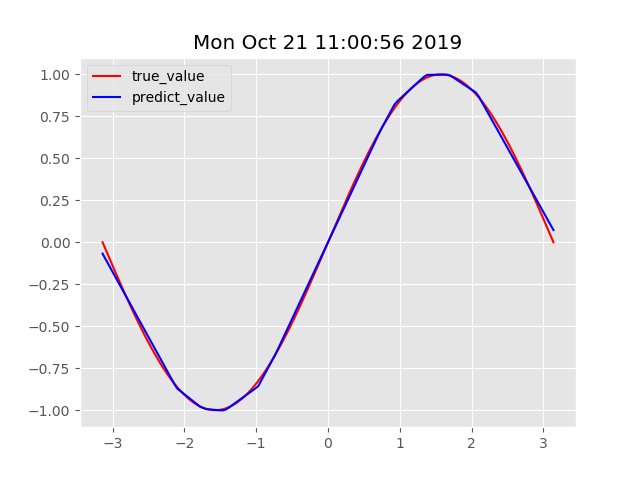
\includegraphics[width=5in]{1.png}
\caption{Output result.}\label{fig1}
\end{figure}

\end{enumerate}
\end{flushleft}


\bibliographystyle{plain}
\bibliography{ref}

\end{document}
%%% Local Variables:
%%% mode: latex
%%% TeX-master: t
%%% End:

%  LocalWords:  headandfoot covariance
